\chapter{Teoretické podklady}
\section{Původ hry}
Čínská dáma má velmi zavádějící název \cite{puvod-cz}. Nepochází z Číny, ale pravděpodobně z Německa nebo Švédska, a s Dámou nemá také v podstatě nic společného. Je velmi podobná Halmě. 

Právě k Halmě může být původ Čínské dámy vysledován \cite{puvod-en}. Jedná se o hru, která byla populární ve Velké Británii v 70. letech 19. století, a která byla založena na starší britské deskové hře zvané \enquote{Hoppity}. Šesticípá hvězda neboli \enquote{Stern} byla v deskové podobě představena v roce 1892 německou herní společností Ravensburger, která hru pojmenovala \enquote{Stern-Halma}. Později, v roce 1928, v~návaznosti na tehdejší světový zájem o orientální mystiku, jako například představení hry Mah Jong v roce 1923 a objevení hrobky krále Tutanchamona v roce 1922, J.~Pressman \& Co. pojmenoval tuto hru \enquote{Čínská dáma}. Hra byla na vrcholku popularity v Americe v 30.\ letech 20.\ století. I přes svou popularitu nebyla ale její minulost zcela zapomenuta, a v Německu, kde se jí stále říká Halma, se hraje podle původních pravidel.

\section{Princip a rozložení hry}
Herní deska Čínské dámy má tvar šesticípé hvězdy \cite{pravidla}. Každý cíp hvězdy je trojúhelník obsahující deset polí (z každé strany je hranice trojúhelníku tvořena čtyřmi poli). Vnitřek desky je hexagon, u něhož je z každé strany jeho hranice tvořena pěti poli. Každý trojúhelník má odlišné zabarvení a~k~dispozici je deset kamenů s odpovídajícími barvami.

Čínská dáma může být hrána dvěma, třemi, čtyřmi nebo šesti hráči \cite{pravidla}. U verze pro šest hráčů budou samozřejmě využity všechny kameny a trojúhelníky. U verze pro čtyři hráče začínají hráči ve dvou párech protilehlých cípů hvězdy, stejně tak u verze pro dva hráče by hráči měli začínat ze dvou protilehlých cípů. U verze pro tři hráče jsou kameny hráčů rozmístěny do tří spolu nesousedících trojúhelníků. Čínská dáma nemůže být hrána pěti hráči \cite{pravidla2}, protože by při takovém počtu hráčů jeden z hráčů bojoval proti prázdné straně hvězdy. Ukázkové počáteční rozložení kamenů na herní desce pro všechny dostupné počty hráčů je možno vidět na obrázku číslo \ref{fig:PocatecniRozlozeni}.

Cílem hry je být prvním hráčem, kterému se podaří přesunout všechny své kameny přes celou herní desku a umístit je do protilehlého cípu \cite{pravidla}. První hráč, kterému se povede obsadit všech deset polí v protilehlém cípu hvězdy, vyhrává. V případě, že více hráčů obsadí protilehlé cípy během stejného tahu, dochází k remíze.

\begin{figure}
	\centering
	\subfloat[2 hráči\label{fig:PocatecniRozlozeni2Hraci}]
	{
		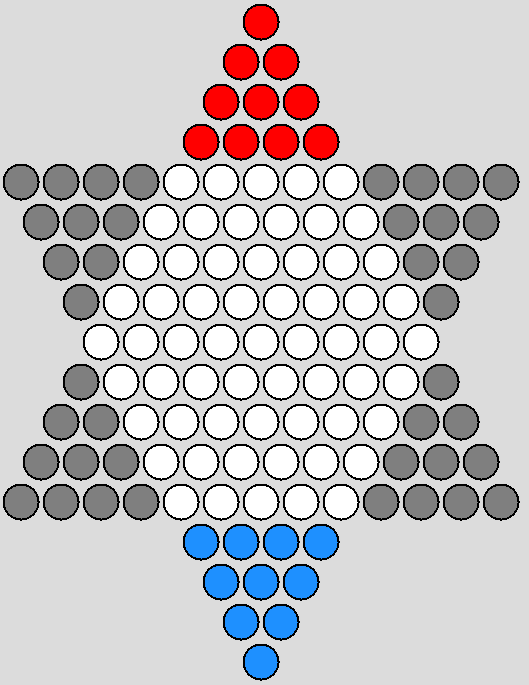
\includegraphics[width=0.35\textwidth]{Figures/PocatecniRozlozeni2Hraci.png}
	}
	\hspace{3em} % make more space
	\subfloat[3 hráči\label{fig:PocatecniRozlozeni3Hraci}]
	{
		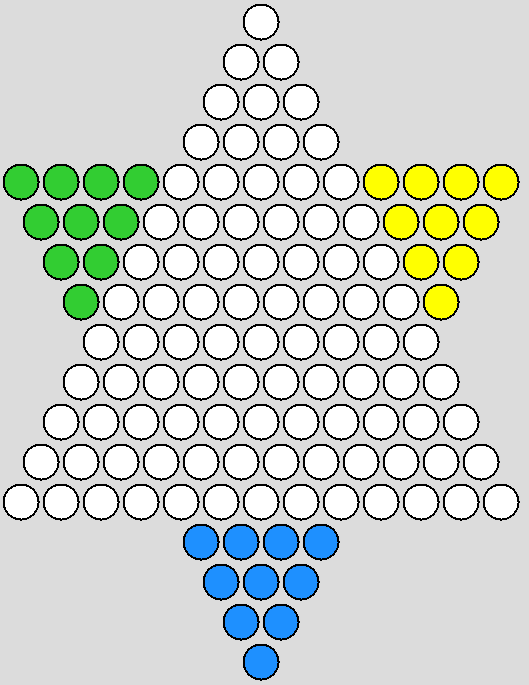
\includegraphics[width=0.35\textwidth]{Figures/PocatecniRozlozeni3Hraci.png}
	}
	\hspace{3em} % make more space
	\subfloat[4 hráči\label{fig:PocatecniRozlozeni4Hraci}]
	{
		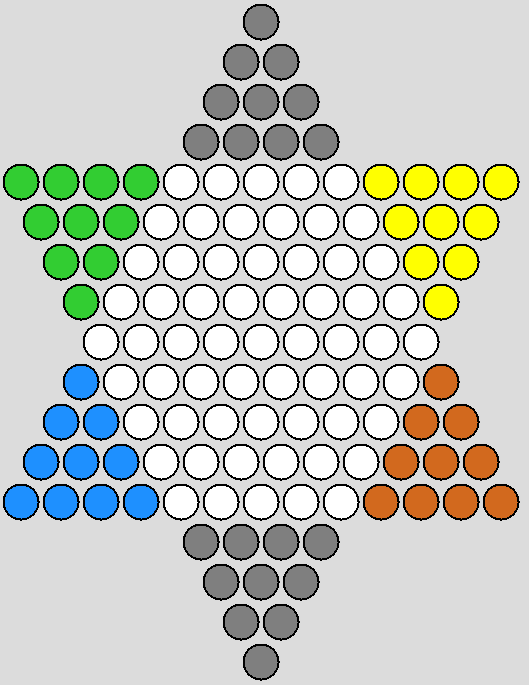
\includegraphics[width=0.35\textwidth]{Figures/PocatecniRozlozeni4Hraci.png}
	}
	\hspace{3em} % make more space
	\subfloat[6 hráčů\label{fig:PocatecniRozlozeni6Hracu}]
	{
		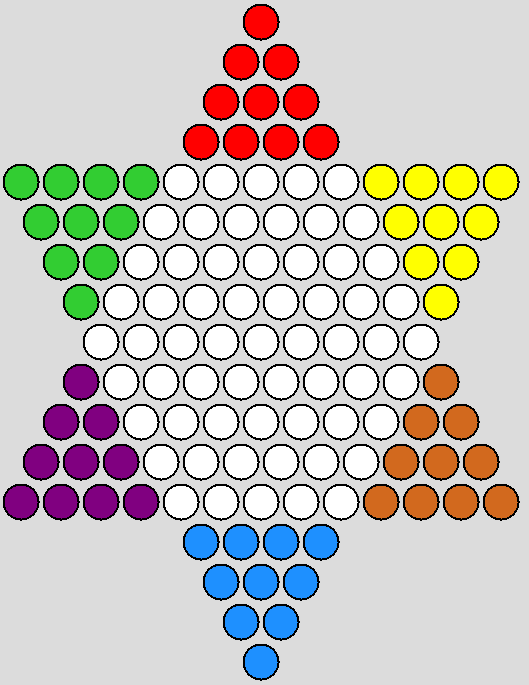
\includegraphics[width=0.35\textwidth]{Figures/PocatecniRozlozeni6Hracu.png}
	}
	\caption[Počáteční rozložení pro všechny dostupné počty hráčů]{Počáteční rozložení pro všechny dostupné počty hráčů (tmavě šedou barvou jsou vyznačena zablokovaná pole)}
	\label{fig:PocatecniRozlozeni}
\end{figure}

\section{Pravidla hry a jejich možné interpretace}
Ohledně pravidel a samotném rozložení hry nepanuje jasná shoda. Jak teoretické popisy, tak praktické implementace hry se od sebe navzájem velmi často liší. Rozdíly mezi jednotlivými verzemi hry jsou sice často pouze v detailech, mnohdy se ale verze hry navzájem liší v důležitých věcech, které zásadním způsobem ovlivňují průběh i výsledek hry. Tato sekce tedy kromě pravidel využívaných ve výsledné implementaci popisuje i další možné interpretace pravidel, se kterými je možné se setkat v dalších popisech a implementacích této hry.

Hráči se mohou mezi sebou dohodnout o tom, kdo z nich bude na tahu jako první \cite{pravidla2}. Pokud se hráči nechtějí o začínajícím hráči dohodnout mezi sebou, je hod mincí jedinou metodou zmíněnou v pravidlech sloužící k ustanovení začínajícího hráče. Následně se hráči v tazích střídají ve směru hodinových ručiček.

Během jednoho tahu přesouvá hráč vždy jediný kámen své barvy. Tyto kameny nelze během průběhu hry žádným způsobem vyřadit ze hry, všechny zůstávají po celou dobu hry na herní desce (na rozdíl od klasické Dámy nebo například šachů, kde k vyřazování kamenů nebo figurek hráčů naopak dochází).

Některé verze pravidel ustanovují, že hráči mohou ovládat více sad kamenů zároveň \cite{pravidla3}. Taková hra je umožněna za předpokladu, že jsou kameny v takovém rozložení, v jakém jsou v naší aplikaci při hře čtyř nebo šesti hráčů. Každý hráč pak ovládá dvě, resp. tři sady kamenů. Vyhrává ten hráč, který jako první přesune všechny své sady kamenů do daných protilehlých trojúhelníků. V rámci této práce má hráč k dispozici vždy jednu sadu kamenů.

Pravidla nejsou jednotná v povolených tazích, podle některých interpretací je možné vždy táhnout na kterékoli pole na desce, podle jiných je možné táhnout pouze na středový hexagon a na výchozí a protilehlý trojúhelník. V této práci byla zvolena varianta pravidel zakazující tahy na hráčské trojúhelníky s výjimkou výchozího trojúhelníku a protilehlého trojúhelníku daného hráče, a to při libovolném počtu hráčů. Zablokovaná (nebo můžeme říct také neaktivní) pole jsou vyznačena tmavě šedou barvou, jejich polohu můžeme vidět na obrázku číslo \ref{fig:PocatecniRozlozeni}.

Vždy panovaly nejasnosti ohledně situace, kdy hráč nemůže vyhrát, protože kámen hráče začínajícího v protilehlém cípu blokuje jedno z polí v daném cípu \cite{pravidla}. Mnohé verze pravidel žádný postup v takové situaci nezmiňují, což by se dalo pochopit tak, že je blokování soupeře tímto pochybným způsobem povoleno. Zde je tato situace vyřešena kontumační výhrou pro blokovaného hráče -- pokud hráč přemístí své kameny do všech volných polí protilehlého cípu a obsadit ta zbývající nemůže výhradně z důvodu, že jsou blokována nepřítelem, je mu udělena kontumační výhra. Tato situace nastává nejčastěji při výrazném dovednostním rozdílu mezi protilehlými hráči, kdy je jeden hráč schopen téměř dokončit hru dříve, než je druhý hráč schopen opustit svůj výchozí trojúhelník. Při testování programu vytvořeného v rámci této práce může tato situace nastat zejména v případě, že jsou do protilehlých cípů proti sobě postaveni počítačoví hráči protipólních obtížností.

Některé interpretace pravidel určují barvy hráčů podle výchozích trojúhelníků hráčů \cite{zapletal}. V této práci má pro přehlednost lidský hráč vždy modrou barvu, nezávisle na tom, který trojúhelník je jeho výchozím. Barvy jednotlivých hráčů budou také přiděleny s ohledem na co nejvyšší vzájemnou odlišitelnost, a to zejména kvůli tomu, že na desce je při každém tahu světlejším odstínem dané barvy vyznačeno pole, ze kterého během tahu daný hráč přesunul kámen.

\section{Možné tahy}
\label{sec:MozneTahy}
Během tahu může hráč kámen přesunout na sousední pole, nebo může provést jeden nebo více skoků přes ostatní kameny \cite{pravidla}. Skok musí být proveden do volného pole, které je za přeskakovaným kamenem, jinak řečeno, musíme být schopni vytvořit jedinou úsečku spojující přesouvaný kámen, přeskakovaný kámen a volné pole, na které chceme doskočit. Každý skok může být proveden přes jakýkoli kámen na herní desce včetně vlastních kamenů. Po každém skoku může hráč buď tah hned ukončit, nebo může pokračovat skokem přes další kámen. Během hry tedy může nastat situace, při které hráč může přesunout kámen z výchozího do protilehlého trojúhelníku v jediném tahu.

Když hráč provádí skok, nesmí být mezi přeskakovaným a přesouvaným kamenem žádný jiný kámen, nelze tedy přeskočit dva a více kamenů během jednoho skoku. Vzdálenost mezi přesouvaným kamenem a přeskakovaným kamenem se musí rovnat vzdálenosti mezi přeskakovaným kamenem a~volným polem, na které chceme doskočit. Mnohé verze pravidel taktéž zmiňují, že po provedení prvního skoku musí být všechny další skoky v rámci daného tahu právě tak dlouhé jako první skok. Na toto pravidlo je při implementaci této práce brán zřetel, délka skoků se tedy v rámci jednoho tahu nemůže lišit.

Zásadní věc, ve které se různé verze pravidel od sebe odlišují, jsou povolené směry tahů. Z~pohledu na herní desku lze určit, že tah lze provést celkem šesti směry (viz obrázek číslo \ref{fig:MozneTahy - Sousedni}). Podle některých názorů je ale zakázáno provádět tahy dozadu, tedy směrem k výchozímu trojúhelníku, což ve výsledku omezí počet povolených směrů na čtyři. V rámci této práce je na toto omezení brán zřetel, a hráči se tak mohou pohybovat všemi šesti směry.

\begin{figure}
	\centering
	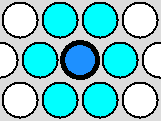
\includegraphics[width=0.4\textwidth]{Figures/MozneTahy - Sousedni.png}
	\caption[Sousední pole, na která je možný přesun]{Sousední pole, na která je možný přesun -- vyznačena světle modře}
    \label{fig:MozneTahy - Sousedni}
\end{figure}

Pro lepší pochopení možných tahů je k dispozici vyobrazení volných polí, na která se hráč může přesunout, zahrnující jak přesuny na sousední pole, tak skoky s různou vzdáleností, na obrázku číslo~\ref{fig:MozneTahy - Skoky}.

\begin{figure}
	\centering
	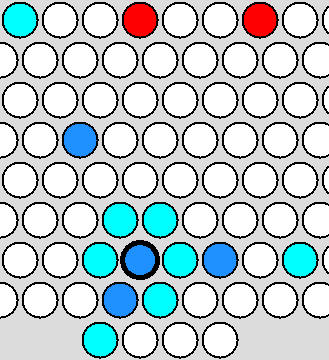
\includegraphics[width=0.4\textwidth]{Figures/MozneTahy - Skoky.png}
	\caption[Pole, na která je možno se přesunout nebo skočit]{Pole, na která je možno se přesunout nebo skočit -- vyznačena světle modře}
    \label{fig:MozneTahy - Skoky}
\end{figure}

\section{Strategie}
\label{sec:Strategie}
Čínská dáma je strategická hra \cite{strategie}, a během její existence tak vymysleli hráči množství strategií, použitelných ve všech fázích hry, jejichž cílem je co nejefektivnější a nejrychlejší přesun všech kamenů do protilehlého trojúhelníku.

Dva nejpoužívanější prvotní tahy jsou Sidewinder a Cross Caterpillar \cite{strategie}. Sidewinder spočívá v~přesunu dvou kamenů nejvzdálenějších od cípu trojúhelníku diagonálně směrem pryč od trojúhelníku. Tato strategie umožní pohyb přes neočekávaná místa, zatímco jiné, často užívané strategie provádějí pohyb přes střed herní desky.

\begin{figure}
	\centering
	\subfloat[tah Sidewinder\label{fig:TahSidewinder}]
	{
		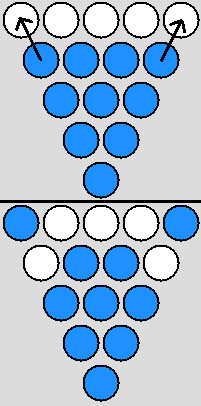
\includegraphics[width=0.35\textwidth]{Figures/PrvotniTahSidewinder.png}
	}
	\hspace{3em} % make more space
	\subfloat[tah Cross Caterpillar\label{fig:TahCrossCaterpillar}]
	{
		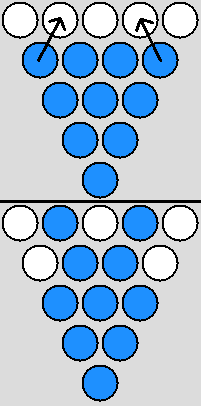
\includegraphics[width=0.35\textwidth]{Figures/PrvotniTahCrossCaterpillar.png}
	}
	\caption{Porovnání nejpoužívanějších prvotních tahů -- Sidewinder a Cross Caterpillar}
	\label{fig:PrvotniTahy}
\end{figure}

Dalším často používaným prvotním tahem je Cross Caterpillar \cite{strategie}. Ten je podobný tahu Sidewinder, s tím rozdílem, že namísto pohybu směrem pryč od trojúhelníku je pohyb proveden směrem ke středu trojúhelníku. Oba tyto tahy jsou velmi efektivní a slouží jako dobrý základ pro další strategické tahy. Porovnání těchto dvou tahů je na obrázku číslo \ref{fig:PrvotniTahy}.

Po provedení prvotních tahů jsou na řadě strategie zaměřené na zbytek hry. Zde jistě stojí za zmínku taktika shlukování \cite{strategie}. Ta je založená na principu vedení kamenů blízko u sebe. Jinak řečeno, hráčovy kameny se přesouvají spolu jako jeden celek, ne jako malé, oddělené skupinky kamenů. Použití této strategie donutí nepřítele k nasměrování svých pohybů kolem kamenů hráče, který tuto taktiku používá. To ve výsledku zpomalí nepřítelův postup, zatímco hráč se postupně stále přibližuje k protilehlému cípu.

Další strategií je blokování \cite{strategie2}. Podle této strategie je nutné neklást důraz pouze na nejvyšší možnou vzdálenost, kterou je možné s kamenem během jednoho tahu urazit, nýbrž je někdy možné získat větší výhodu zablokováním soupeře, a to bez ohledu na vzdálenost mezi kamenem a cílovým polem. Mnohdy je takto nazýváno úmyslné ponechání kamene ve výchozím trojúhelníku, což ve výsledku znemožní hráči z protilehlého cípu dokončit hru. Této taktice se také říká \enquote{spoiling} a je obecně považována za pochybnou.

Strategií určenou pro středovou fázi hry je postavení mostu \cite{strategie}. Tento most umožní hráči efektivně přesouvat kameny z jednoho konce desky na druhý. Je ale nutné mít na paměti, že nepřítel bude také mít možnost využívat tento most. Je proto nutné se proti této možnosti bránit například využitím blokování. Na obrázku číslo \ref{fig:Most} je k nahlédnutí ukázka jednoduchého mostu, který může být vybudován během čtyř tahů.

\begin{figure}
	\centering
	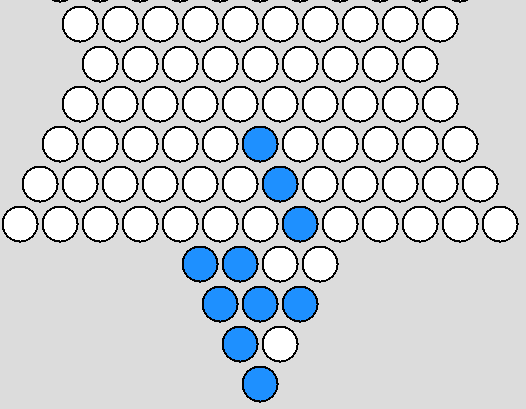
\includegraphics[width=0.4\textwidth]{Figures/Most.png}
	\caption{Ukázka strategie postavení mostu}
    \label{fig:Most}
\end{figure}

V závěrečné fázi hry, kdy hráč začne obsazovat protilehlý trojúhelník, je výhodné nejprve obsadit hrany tohoto pomyslného trojúhelníku \cite{strategie2}, a až poté jeho středové části. Tento postup mírně ulehčí přesunutí zbývajících kamenů do cílového trojúhelníku.
\endinput